\documentclass[11pt,a4paper]{article}
\usepackage[T1]{fontenc}
\usepackage{lmodern}
\usepackage[margin=27mm,headheight=14pt]{geometry}
\usepackage{amsmath,amssymb,amsthm,mathtools,bm}
\usepackage{microtype,booktabs,longtable,array,enumitem}
\usepackage{graphicx,hyperref,fancyhdr,xurl}
\hypersetup{hidelinks,pdftitle={Theta-Resolved Optimal Truncation of q-Multinomial Transseries},pdfauthor={OpenAI; prepared for Vladimir Reshetnikov}}
\pagestyle{fancy}\fancyhf{}
\fancyhead[L]{\small Theta-resolved optimal truncation}
\fancyhead[R]{\small Research manuscript}
\fancyfoot[C]{\thepage}
\setlength{\parskip}{3pt}
\setlength{\emergencystretch}{3em}
\numberwithin{equation}{section}
\newtheorem{theorem}{Theorem}[section]
\newtheorem{proposition}[theorem]{Proposition}
\newtheorem{lemma}[theorem]{Lemma}
\newtheorem{corollary}[theorem]{Corollary}
\theoremstyle{definition}\newtheorem{definition}[theorem]{Definition}
\newtheorem{example}[theorem]{Example}
\theoremstyle{remark}\newtheorem{remark}[theorem]{Remark}
\newcommand{\e}{\mathrm e}
\newcommand{\dd}{\,\mathrm d}
\newcommand{\R}{\mathbb R}
\newcommand{\N}{\mathbb N}
\newcommand{\Z}{\mathbb Z}
\newcommand{\avec}{\boldsymbol a}
\newcommand{\astar}{a_*}
\newcommand{\mstar}{m_*}
\newcommand{\eps}{\varepsilon}
\newcommand{\calE}{\mathcal E}
\newcommand{\calJ}{\mathcal J}
\newcommand{\calM}{\mathcal M}
\newcommand{\calP}{\mathcal P}
\newcommand{\calA}{\mathcal A}
\DeclareMathOperator{\Li}{Li}
\DeclareMathOperator{\dist}{dist}
\DeclareMathOperator{\Var}{Var}
\DeclareMathOperator{\argmin}{argmin}
\title{\textbf{Theta-Resolved Optimal Truncation\ of $q$-Multinomial Transseries}\\[7pt]
\large A phase-dependent $\sqrt{x}$ shift, arithmetic error actions,\\
and an exact hierarchy of pole-resolved approximations}
\author{Research manuscript prepared for Vladimir Reshetnikov\\\small OpenAI}
\date{29 September 2026}
\begin{document}
\maketitle
\begin{abstract}
The positive-remainder approach to $q$-multinomial asymptotics leaves a
specific question: how does a continuous least-remainder saddle turn into
an arithmetic lattice saddle? We give a uniform, all-order answer when the
lattice spacing is bounded in units of the saddle width. More importantly,
we distinguish a conventional least-term rule from the \emph{actual}
minimization over all Bernoulli truncation orders. The latter is governed
by a tilted Gaussian lattice sum. If $z=a_*x$, $\beta=2\pi$,
$\lambda=h\sqrt{z/\beta}$ and $\theta=\{\beta/h\}$, then
\[
  2K_{\min}=\beta z+\eta_*(\lambda,\theta)\sqrt{\beta z}+O(1),
\]
where $\eta_*$ is the unique tilt making the lattice mean zero. The minimum
remainder has leading value
$\frac{m_*\sqrt{2\pi}}{\beta^{3/2}\sqrt z}\e^{-\beta z}
\min_\eta\calJ_\lambda(\theta,\eta)$.
We also calculate the bounded correction to the continuously optimal order
and the first correction to the minimum itself.

For fixed nonresonant $0<h<\beta$, the optimal error instead has an exact
arithmetic action $I_h>\beta$, determined by the two lattice points
straddling $\beta$. Its prefactor retains an oscillation from the integer
truncation order. A mesoscopic theorem matches this two-point law to the
large-mesh theta law. Finally, resolving the first $L$ partial-fraction
poles exactly replaces $\beta$ by $2\pi(L+1)$ throughout the critical-mesh
theory. Explicit positive tail bounds turn these representations into
finite forward and inverse error certificates.

The article supplies conventional proofs, symbolic checks, and numerical
diagnostics. The claims are scoped extensions of the inspected ProveIt
transseries program and of an earlier research draft, not a claim to have
settled general resurgence or established literature-wide priority.
\end{abstract}
\medskip
\noindent\textbf{Status.} Unrefereed mathematical development. No Lean build,
interval-arithmetic validation, or independent peer review is claimed.
\clearpage
{\small\setlength{\parskip}{0pt}\tableofcontents}
\clearpage

\section{Research target, contribution, and source boundary}
\label{sec:scope}

\subsection{The problem being advanced}
The ProveIt series-and-transseries corpus develops polynomial--logarithmic
calculus, exact-core inversion, and asymptotic expansions of rapidly growing
combinatorial families. Its companion on combinatorial transseries includes
Gaussian coefficients and the singular $q\to1$ transition
\cite{repo,repo-group,repo-canonical}. A preceding research draft,
\emph{Uniform $q$-Multinomial Transseries and Certified Inversion}
\cite{prior}, obtains a positive exact remainder for every positive
multinomial ray. Its final section explicitly proposes two further targets:
a lattice-to-integral transition formula, including the fractional saddle
position, and a first resolved beyond-all-orders correction. Those are the
immediate targets here.

The distinction between the sources matters. The preceding draft was read
from the user's saved research files; it is not being represented as a
verified publication or as a file proved to be present in the current
repository. The repository's directly retrieved transseries READMEs were
pinned at commit \texttt{ae28ea2db3c01a0b777cffa6295b8fe9c4628f27}.
Current directory listings were also inspected, but the large canonical
source exceeded the available file endpoint. Therefore this is a targeted
extension, not an exhaustive nonduplication audit of the entire current
repository. The exact mathematical starting formulas are restated and
proved below, so the new theorems do not depend on trusting the earlier
draft's correctness.

The previous two sharp special cases have an instructive contrast. At
$h=0$, the ordinary near-least-term remainder has a factor $z^{-1/2}$.
At $h=2\pi/m$, a lattice point lands exactly on the saddle and that factor
is absent. Simply replacing a sum by an integral misses this difference.
The appropriate intermediate object is a Gaussian lattice sum rather than
a Gaussian integral.

There is a second distinction, not resolved merely by finding that sum:
minimizing a convenient envelope is not the same as minimizing the exact
remainder. At a nonsymmetric lattice phase, an order displacement of size
$\sqrt z$ changes the relative weights of the nearby lattice points by an
order-one amount. Consequently a rule $2K=2\pi z+O(1)$ can have the right
exponential scale and still miss the best leading constant. At fixed
nonresonant $h$, it can even miss the optimal exponential action.

% ed. (2026-09-29): editorial note added by ProveIt (the preceding draft
% is now filed; sibling packages; uncited repository results); not part of
% the delivered text.
\begin{quote}\small
\textbf{Editorial note (ProveIt, 2026-09-29).}
The preceding draft \cite{prior} is now filed in the repository as
\path{Uniform_q_Multinomial_Certified_Inversion/uniform_q_multinomial_transseries.tex}
\cite{ed:siblings}. As delivered it had the 1,521 lines and the four labels
that this article names; at its questions Q1 and Q2 (section ``Further
research questions and topics'') an editorial note now points here and
states the scope of the answers given here. This article belongs to a unit of five
packages that answer the companion's $q\to1$ gap for the same interpolation
and are to be merged into its chapter on the singular transition
\cite{ed:siblings}: the preceding draft, the central Gaussian-binomial,
certified-inversion and gamma-core articles, and this article.
The five write the interpolation in different normalizations ($q=\e^h$ or $Q=\e^{-h}$; remainders $R_K$, $r_K$, $R_M$ or $L_h-F_{h,K}$; smallest ray parameter $a_*$, $\alpha$ or $a_{\min}$); a normalization dictionary is left to the merge.
The same restriction $\tau\ge\tau_0$ appears in Theorem
\texttt{q3:thm:double-scaling} of the Fabius tree's Gaussian-coefficient
volume \cite{ed:gcc}, which the preceding draft's uniform theorem removes;
neither article cites it. Theorems~\ref{thm:optimal} and
\ref{thm:hierarchy} are sharp, theta-resolved instances of the canonical
volume's least-term theorem \texttt{p0:thm:optimal-truncation}
\cite{ed:tai}, and Theorem~\ref{thm:inverse} uses the residual-to-root step
that the Lean theorem \path{Fabius.exists_eq_in_residual_interval}
\cite{ed:lean} checks in abstract form; this article cites neither.
\end{quote}

\subsection{What is new in the present development}
The central results are the following, in increasing order of refinement.
\begin{enumerate}[label=(\roman*),leftmargin=2em]
\item Theorem~\ref{thm:theta} gives an all-order expansion of the exact
remainder, uniform for bounded saddle-scaled mesh and bounded order tilt.
\item Theorem~\ref{thm:optimal} minimizes over \emph{all} integer orders.
It determines the $\sqrt z$ displacement, its bounded correction, and the
first correction to the minimum error.
\item Theorem~\ref{thm:fixed} identifies the exact fixed-mesh action and the
remaining integer-order oscillation. Theorem~\ref{thm:overlap} rigorously
matches it with the theta description in an overlapping regime.
\item Theorem~\ref{thm:hierarchy} applies the same analysis after any fixed
number of poles have been resolved exactly. Theorem~\ref{thm:finite}
supplies finite evaluation bounds; Theorem~\ref{thm:inverse} transports them
to inverse errors.
\end{enumerate}
The words ``all-order'' always refer to a finite-order asymptotic statement
for every fixed requested order. They do not assert convergence of the
infinite saddle expansion.

\subsection{Classical mechanisms and the novelty claim}
The ingredients are not new in isolation. The partial fractions of $\coth$,
Binet's integral, $q$-gamma limits, and theta transformations are classical
\cite{dlmf-hyperbolic,dlmf-gamma,dlmf-qgamma,dlmf-theta}. Discrete Laplace
methods have a substantial history; a recent systematic treatment is due
to Hughes, Helton, and Schlosser \cite{discrete-laplace}. The resurgence of
Euler--Maclaurin summation and quantum dilogarithms has been studied by
Costin--Garoufalidis and Garoufalidis--Kashaev
\cite{costin-garoufalidis,garoufalidis-kashaev}.

The contribution advanced here is the \emph{specific quantified package}:
the positive $q$-multinomial remainder, its phase-dependent global
minimization, the arithmetic action and order oscillation, and the reusable
pole-resolved hierarchy. We do not claim priority for theta asymptotics,
optimal truncation, or resurgence as general subjects. The literature check
identifies relevant precedents but does not establish that no equivalent
specialized theorem exists elsewhere. None of the new proofs uses a
hypothesis of general Borel summability.

\section{The analytic family and its exact positive remainder}
\label{sec:family}

Fix $r\ge2$ and a positive ray $\avec=(a_1,\ldots,a_r)$. Throughout, set
\begin{equation}
 A=\sum_{j=1}^r a_j,\quad d=r-1,\quad
 \kappa=\frac{A^2-\sum_j a_j^2}{2},\quad
 \astar=\min_j a_j,\quad
 \mstar=\#\{j:a_j=\astar\},\quad z=\astar x.
 \label{eq:parameters}
\end{equation}
In every uniform assertion the ray is fixed. Uniformity as its entries
coalesce or tend to zero is a separate problem.

For $h>0$, define
\begin{align}
 \calP(h)&=\prod_{n\ge1}(1-\e^{-hn}),\label{eq:product}\\
 \calA_h(s)&=\sum_{m\ge1}\frac{\e^{-ms}}{m(\e^{hm}-1)},\qquad s>0,\\
 F_h(x)&=\kappa hx^2-d\log\calP(h)
       +\calA_h(Ahx)-\sum_j\calA_h(a_jhx),\quad x>0.
 \label{eq:F}
\end{align}
At $h=0$, put
\begin{equation}
 F_0(x)=\log\Gamma(Ax+1)-\sum_j\log\Gamma(a_jx+1).
 \label{eq:Fzero}
\end{equation}
When all $a_jx$ are integers, $\exp F_h(x)$ is the Gaussian multinomial
coefficient at $q=\e^h$. For general ray entries, \eqref{eq:F} specifies the
interpolation being studied. There is no assertion about arbitrary
interpolations of the same integer sequence.

To check the endpoint, let $Q=\e^{-h}$. The product definition of
$\Gamma_Q$ gives
\begin{equation}
 \e^{F_h(x)}=\e^{\kappa hx^2}
 \frac{\Gamma_Q(Ax+1)}{\prod_j\Gamma_Q(a_jx+1)}.
 \label{eq:qgamma}
\end{equation}
The powers of $1-Q$ cancel because $A=\sum_j a_j$.
The classical limit $\Gamma_Q(u)\to\Gamma(u)$ for positive $u$ proves
$F_h(x)\to F_0(x)$ for each fixed $x>0$ \cite{dlmf-qgamma}.

\subsection{A finite Bernoulli expansion}
Write $b=2\pi$ and $b_\ell=b\ell$. The positive multinomial weight is
\begin{equation}
 W(s)=\sum_j\e^{-a_js}-\e^{-As}>0\quad(s\ge0).
 \label{eq:W}
\end{equation}
It satisfies $W(s)\le r\e^{-\astar s}$, and its leading large-$s$ term is
$\mstar\e^{-\astar s}$. Let
\begin{equation}
 c_k=\frac{B_{2k}}{(2k)!},\qquad
 V_\nu(\tau)=\Li_\nu(\e^{-A\tau})-\sum_j\Li_\nu(\e^{-a_j\tau}).
\end{equation}
For $h>0$, define
\begin{align}
 \Phi_h(x)&=\kappa hx^2-d\log\calP(h)
       +h^{-1}V_2(hx)-\tfrac12 V_1(hx),\\
 T_K(h,x)&=\Phi_h(x)+\sum_{k=1}^K c_kh^{2k-1}V_{2-2k}(hx),
 \quad K\in\N\cup\{0\}.
 \label{eq:TK}
\end{align}
The exact product in $\Phi_h$ is retained. In particular, exponentially
small modular information in that product has not been discarded.
At the endpoint use
\begin{align}
 H_{\avec}&=A\log A-\sum_j a_j\log a_j,\\
 \Phi_0(x)&=H_{\avec}x-\tfrac d2\log(2\pi x)
                     +\tfrac12\log\frac{A}{\prod_j a_j},\\
 T_K(0,x)&=\Phi_0(x)+\sum_{k=1}^K
 \frac{B_{2k}}{2k(2k-1)}
 \frac{A^{1-2k}-\sum_j a_j^{1-2k}}{x^{2k-1}}.
 \label{eq:Tzero}
\end{align}
These are finite sums even when $K$ depends on $x$.

It is convenient to write both lattice and continuous formulas using a
positive measure:
\begin{equation}
 \int f(t)\dd\nu_h(t)=
 \begin{cases}
 h\displaystyle\sum_{m\ge1}f(hm),&h>0,\\
 \displaystyle\int_0^\infty f(t)\dd t,&h=0.
 \end{cases}
 \label{eq:measure}
\end{equation}

\begin{proposition}[Exact signed remainder]
\label{prop:remainder}
For $x>0$, $h\ge0$ and $K\ge0$,
\begin{equation}
 F_h(x)-T_K(h,x)=(-1)^{K+1}\calE_0(2K;h,x),
 \label{eq:remainder}
\end{equation}
where, more generally for $L\ge0$ and $p\ge0$,
\begin{equation}
 \calE_L(p;h,x)=2\int_0^\infty W(xt)
      \sum_{\ell=L+1}^\infty
      \frac{(t/b_\ell)^p}{b_\ell^2+t^2}\dd\nu_h(t)>0.
 \label{eq:E}
\end{equation}
All displayed integrals and sums converge absolutely. They can be
repeatedly differentiated in $p$ on compact subsets of $p>-1$.
\end{proposition}
\begin{proof}
The partial fractions of $\coth$ \cite{dlmf-hyperbolic} give
\[
 \frac1{\e^v-1}=\frac1v-\frac12+
       2v\sum_{\ell\ge1}\frac1{b_\ell^2+v^2}.
\]
Apply the finite identity
\begin{equation}
 \frac1{b_\ell^2+v^2}
 =\sum_{j=0}^{K-1}\frac{(-1)^jv^{2j}}{b_\ell^{2j+2}}
    +\frac{(-1)^Kv^{2K}}{b_\ell^{2K}(b_\ell^2+v^2)}.
 \label{eq:geometric}
\end{equation}
The Bernoulli coefficient identity
$c_k=2(-1)^{k-1}\zeta(2k)/(2\pi)^{2k}$ identifies the finite terms.
In \eqref{eq:F}, the remaining kernel is multiplied by $-W(mhx)/m$.
Since $v=hm$, this is exactly \eqref{eq:remainder} for $h>0$.

For $h=0$, Binet's integral \cite{dlmf-gamma} in the form
\[
 \log\Gamma(u+1)=\left(u+\tfrac12\right)\log u-u
 +\tfrac12\log(2\pi)
 +\int_0^\infty\frac{\e^{-ut}}t
 \left(\frac1{\e^t-1}-\frac1t+\frac12\right)\dd t
\]
produces the same expression after taking the gamma quotient and applying
\eqref{eq:geometric}. Near zero, $t^p|\log t|^j$ is integrable for $p>-1$.
At infinity the ray weight decays exponentially, and the pole sum is
bounded by a constant multiple of $\sum\ell^{-p-2}$ on compact $p$ ranges.
These bounds, with logarithmic factors included, justify the assertions
about convergence and differentiation. Positivity follows from
\eqref{eq:W}.
\end{proof}

\subsection{Resolving finitely many poles exactly}
Define
\begin{equation}
 T_{K,L}(h,x)=T_K(h,x)+(-1)^{K+1}2\int W(xt)
    \sum_{\ell=1}^{L}\frac{(t/b_\ell)^{2K}}{b_\ell^2+t^2}\dd\nu_h(t).
 \label{eq:resolved}
\end{equation}
The sum is empty at $L=0$. Proposition~\ref{prop:remainder} immediately gives
\begin{equation}
 F_h(x)-T_{K,L}(h,x)=(-1)^{K+1}\calE_L(2K;h,x).
 \label{eq:resolved-error}
\end{equation}
Resolving a pole here means evaluating its positive remainder component,
not appending a guessed exponential coefficient. Put
\begin{equation}
 \beta=b(L+1),\qquad
 C_\beta(z)=\frac{\mstar\sqrt{2\pi}}{\beta^{3/2}\sqrt z}.
 \label{eq:beta}
\end{equation}
All subsequent theorems allow an arbitrary fixed $L$. The case $L=0$ is
the original Bernoulli truncation problem.

\section{Gaussian lattice sums and the zero-mean tilt}
\label{sec:theta}

For $\lambda>0$, $\theta\in\R/\Z$ and $\eta\in\R$, let
\begin{align}
 u_k&=\lambda(k-\theta),\\
 \calJ_\lambda(\theta,\eta)
 &=\frac{\lambda}{\sqrt{2\pi}}
       \sum_{k\in\Z}\exp(-u_k^2/2+\eta u_k),\label{eq:J}\\
 M_j(\lambda,\theta,\eta)
 &=\frac{\lambda}{\sqrt{2\pi}}
       \sum_{k\in\Z}u_k^j\exp(-u_k^2/2+\eta u_k).
 \label{eq:moments}
\end{align}
Thus $M_j=\partial_\eta^j\calJ$. At $\lambda=0$, replace the normalized
sum by the normalized Gaussian integral on $\R$; in particular,
$\calJ_0(\theta,\eta)=\e^{\eta^2/2}$. The phase is irrelevant at that
endpoint.

Let $\Theta_\lambda(\theta)=\calJ_\lambda(\theta,0)$. Completing the square
and applying Gaussian Poisson summation give
\begin{align}
 \calJ_\lambda(\theta,\eta)
 &=\e^{\eta^2/2}\Theta_\lambda(\theta+\eta/\lambda),\label{eq:shift}\\
 \Theta_\lambda(\theta)
 &=\sum_{n\in\Z}\e^{-2\pi^2n^2/\lambda^2}\e^{2\pi i n\theta}
 =1+2\sum_{n\ge1}\e^{-2\pi^2n^2/\lambda^2}\cos(2\pi n\theta).
 \label{eq:poisson}
\end{align}
This is the standard Gaussian instance of the theta transformation
\cite{dlmf-theta}. It also follows directly by computing the Fourier
coefficients of the periodic Gaussian sum. The real Gaussian sum is useful
for large $\lambda$; its Fourier form is useful for small $\lambda$.

\begin{lemma}[Uniform Gaussian lattice control]
\label{lem:gaussian}
Fix $H,M<\infty$ and a nonnegative integer $j$. The moments in
\eqref{eq:moments}, and any fixed number of their $\eta$ derivatives, are
uniformly bounded for
\[
 0\le\lambda\le H,\qquad\theta\in\R/\Z,\qquad |\eta|\le M.
\]
The normalized sums of $(1+|u|^j)\e^{-c u^2+M|u|}$ are also bounded for
any fixed $c>0$. They have the corresponding integral limit uniformly in
$\theta$ as $\lambda\downarrow0$.
\end{lemma}
\begin{proof}
Partition the real line into unit intervals. An interval contains at most
$1+1/\lambda$ lattice points, so its normalized counting mass is at most
$1+H$. The suprema of the Gaussian envelope on these intervals form a
summable sequence. This proves domination, including polynomial factors.
For the limit, first truncate to a compact interval. The shifted Riemann
sums of a uniformly continuous function converge uniformly in their shifts.
The dominated Gaussian tails are arbitrarily small uniformly in $\lambda$.
Differentiation in $\eta$ only adds polynomial factors.
\end{proof}

\begin{proposition}[The minimizing tilt]
\label{prop:tilt}
For each $\lambda\ge0$ and each phase $\theta$, $\calJ_\lambda(\theta,\eta)$
has a unique minimizer $\eta_*=\eta_*(\lambda,\theta)$, characterized by
\begin{equation}
 M_1(\lambda,\theta,\eta_*)=0.
 \label{eq:zeromean}
\end{equation}
Define
\begin{equation}
 \calM_\lambda(\theta)=\calJ_\lambda(\theta,\eta_*).
 \label{eq:Mprofile}
\end{equation}
On every bounded interval $0\le\lambda\le H$, $\eta_*$ is bounded,
$\calM_\lambda$ is bounded away from zero, and
$M_2(\lambda,\theta,\eta_*)$ is bounded away from zero, uniformly in
$\theta$. These functions are continuous with their endpoint values.
At $\lambda=0$, $\eta_*=0$ and $\calM_0=1$.
\end{proposition}
\begin{proof}
The second $\eta$ derivative is $M_2>0$: the lattice has points other than
zero, all with positive weights. The integral case has the same property.
There is positive mass on both positive and negative half-lines, so the
function tends to infinity as $\eta\to\pm\infty$. This gives existence,
strict uniqueness, and \eqref{eq:zeromean}.

For uniformity, choose positive and negative compact intervals separated
from zero, each long enough to contain several points of every lattice
with $\lambda\le H$. Their normalized Gaussian masses have positive lower
bounds. The contributions from the interval of the same sign as $\eta$
grow exponentially as $|\eta|$ grows; the opposite-sign derivative
contribution is uniformly bounded and then decays. Hence the derivative
has opposite signs at $\eta=\pm M_H$ for some fixed $M_H$. Lemma~\ref{lem:gaussian}
and the implicit function theorem now give continuity of the zero and
of the moments on the compact parameter set. Strict positivity and
compactness give both lower bounds. The limiting statements also follow
from \eqref{eq:poisson} and \eqref{eq:shift}.
\end{proof}

The condition \eqref{eq:zeromean} has a simple interpretation: the optimal
order reweights the lattice so that its weighted displacement from the
continuous saddle is zero. At phases $0$ and $1/2$, symmetry makes the
optimal tilt zero. At a general phase it need not vanish. For example,
the included numerical calculation at $(\lambda,\theta)=(4,1/4)$ gives
\begin{equation}
 \eta_*\approx0.725347327957,\qquad
 \calM_4(1/4)\approx0.624809319319.
 \label{eq:example-tilt}
\end{equation}
These decimal values are diagnostics; their defining equations are exact.

\section{The all-order critical-mesh theorem}
\label{sec:allorder}

Let $L$ and the ray be fixed. For $h>0$, introduce
\begin{equation}
 \lambda=h\sqrt{z/\beta},\qquad
 \theta=\{\beta/h\},\qquad
 \eps=(\beta z)^{-1/2},\qquad
 p=\beta z+\eta\sqrt{\beta z}.
 \label{eq:scaling}
\end{equation}
At $h=0$, set $\lambda=0$ and any phase $\theta$. The saddle coordinate is
$u=(t-\beta)\sqrt{z/\beta}$, so $t=\beta(1+\eps u)$.
For a lattice point $t=hm$, its $u$ coordinate lies in
$\lambda(\Z-\theta)$.

Define polynomials $P_j(u,\eta)$ by the formal expansion
\begin{align}
 \sum_{j\ge0}P_j(u,\eta)\eps^j
 ={}&\frac{2}{1+(1+\eps u)^2}\notag\\[-2pt]
 &\times\exp\left\{
 \frac{\log(1+\eps u)-\eps u+(\eps u)^2/2}{\eps^2}
 +\eta\left(\frac{\log(1+\eps u)}\eps-u\right)\right\}.
 \label{eq:Pgen}
\end{align}
The apparent singularities in $\eps$ are removable as formal series.
Each $P_j$ is a finite polynomial. In particular,
\begin{align}
 P_0={}&1,\notag\\
 P_1={}&\frac{u^3}{3}-\frac{\eta u^2}{2}-u,\label{eq:P1}\\
 P_2={}&\frac{u^2}{2}+\frac{5\eta u^3}{6}
 +\left(\frac{\eta^2}{8}-\frac7{12}\right)u^4
 -\frac{\eta u^5}{6}+\frac{u^6}{18}.
 \label{eq:P2}
\end{align}
Let
\begin{equation}
 \calJ_{j,\lambda}(\theta,\eta)
 =\frac{\lambda}{\sqrt{2\pi}}
 \sum_{k\in\Z}\e^{-u_k^2/2+\eta u_k}P_j(u_k,\eta),
 \label{eq:Jj}
\end{equation}
with its Gaussian integral interpretation at $\lambda=0$.
Thus $\calJ_{0,\lambda}=\calJ_\lambda$.

\begin{theorem}[Uniform theta expansion]
\label{thm:theta}
Fix $L\ge0$, the positive ray $\avec$, $H,M<\infty$, and integers $J,q\ge0$.
As $z\to\infty$,
\begin{equation}
 \frac{\calE_L(p;h,x)}{C_\beta(z)\e^{-\beta z}}
 =\sum_{j=0}^{J}\eps^j\calJ_{j,\lambda}(\theta,\eta)
       +O_{\avec,L,H,M,J,q}(\eps^{J+1}),
 \label{eq:allorder}
\end{equation}
uniformly for $h\ge0$ with $0\le\lambda\le H$ and $|\eta|\le M$.
The same estimate holds after any number at most $q$ of $\eta$ derivatives,
where $h,x$ are held fixed while $p$ varies as in \eqref{eq:scaling}.
\end{theorem}

\subsection{Isolating the first pole and the smallest ray}
We give the estimates behind the uniform assertion rather than treating
the moving lattice as an informal Riemann sum.

\begin{lemma}[Unimodal sum bound]
\label{lem:unimodal}
If $f\ge0$ is integrable and unimodal on $(0,\infty)$, then
\begin{equation}
 \int f\dd\nu_h\le\int_0^\infty f(t)\dd t+h\sup f,
 \qquad h>0.
 \label{eq:unimodal}
\end{equation}
For $f(t)=t^p\e^{-zt}$ with $p\ge0$, this gives
\begin{equation}
 \int f\dd\nu_h\le\frac{\Gamma(p+1)}{z^{p+1}}
                 +h\left(\frac{p}{\e z}\right)^p,
 \label{eq:moment}
\end{equation}
where the last power equals $1$ when $p=0$.
\end{lemma}
\begin{proof}
On the increasing side, compare each lattice value with the integral on
the interval to its right. On the decreasing side, use the interval to
its left. These intervals are disjoint except for the single interval
straddling the maximum. Accounting for that one value costs at most
$h\sup f$. This proves \eqref{eq:unimodal}; the gamma integral and the
maximum at $p/z$ give \eqref{eq:moment}.
\end{proof}

\begin{lemma}[Exponential separation]
\label{lem:separation}
In the regime of Theorem~\ref{thm:theta}, there is $c>0$ such that
\begin{equation}
 \calE_L(p;h,x)=
 2\mstar\int\frac{(t/\beta)^p\e^{-zt}}{\beta^2+t^2}\dd\nu_h(t)
 +O\bigl(C_\beta(z)\e^{-\beta z-cz}\bigr).
 \label{eq:firstpole}
\end{equation}
The assertion remains valid after any fixed number of $\eta$ derivatives,
possibly with a smaller $c$.
\end{lemma}
\begin{proof}
For a later pole $b_\ell>\beta$, its integrand divided by the first-pole
integrand is at most $(\beta/b_\ell)^p$. For $p=\beta z+O(\sqrt z)$,
\[
 \sum_{\ell\ge L+2}(\beta/b_\ell)^p
 \le\left(\frac{L+1}{L+2}\right)^p
        \left(1+\frac{L+2}{p-1}\right),
\]
which is exponentially small. The bound follows by comparing the decreasing
power tail with an integral.

For a ray parameter $a>\astar$, set $\alpha=a/\astar>1$. Its first-pole
contribution has the upper bound
\[
 2\beta^{-p-2}\int t^p\e^{-\alpha zt}\dd\nu_h(t).
\]
By \eqref{eq:moment} and Stirling's formula, its ratio to
$C_\beta(z)\e^{-\beta z}$ is bounded by a polynomial in $z$ times
$\exp(-\beta z\log\alpha+O(\sqrt z))$. The same estimate applies to the
negative numerator term with $a=A$. There are finitely many such parameters.
For the smallest ray, \eqref{eq:moment} gives the required order upper bound
on the first-pole contribution because $h=O(z^{-1/2})$. The claimed separation
follows by decreasing $c$ to absorb polynomial factors.

A $\eta$ derivative multiplies an integrand by
$\sqrt{\beta z}\log(t/b_\ell)$. Any fixed power of this factor is handled by
splitting $t$ into $(0,\beta/2)$, $[\beta/2,2\beta]$, and $(2\beta,\infty)$
and using the same exponential moments. Equivalently, bound logarithmic
powers by a small positive or negative power of $t$ and $\ell$; such fixed
changes do not alter a strict exponential gap.
\end{proof}

\subsection{Proof of Theorem~\ref{thm:theta}}
By Lemma~\ref{lem:separation}, only the first term in \eqref{eq:firstpole}
needs expansion. Substitution of $t=\beta(1+\eps u)$ gives its normalized
form exactly as
\begin{equation}
 \frac\lambda{\sqrt{2\pi}}
 \sum_{u\in\lambda(\Z-\theta),\ u>-1/\eps}
 \e^{-u^2/2+\eta u}Q_\eps(u,\eta),
 \label{eq:exact-scaled}
\end{equation}
where $Q_\eps$ is the right side of \eqref{eq:Pgen}. At $h=0$ this is the
corresponding integral. The normalization uses
$h\sqrt{z/\beta}=\lambda$ and is therefore valid without a limiting
approximation of the lattice.

First restrict to $|u|\le\eps^{-1/12}$. Taylor's theorem applied to the
logarithm, the exponential, and the rational prefactor shows, for every
fixed $J$, that
\begin{equation}
 \left|Q_\eps-\sum_{j=0}^J\eps^jP_j\right|
 \le C\eps^{J+1}(1+|u|^{D_J})\e^{c_0\eps |u|^3+c_1\eps u^2}.
 \label{eq:taylor-dom}
\end{equation}
Here $D_J$ is a finite integer; the constants can be chosen uniformly for
bounded $\eta$. The same form holds for finitely many $\eta$ derivatives.
On the chosen region the extra exponential is bounded by a Gaussian
factor that leaves, for sufficiently small $\eps$, a majorant
$C(1+|u|^{D})\e^{-u^2/4+M|u|}$. Lemma~\ref{lem:gaussian} therefore makes the
summed or integrated error $O(\eps^{J+1})$.

For completeness, the complement is negligible uniformly in the mesh.
On $t/\beta\in[1/2,2]$, the function
$\log(t/\beta)-t/\beta+1$ is bounded above by
$-c(t/\beta-1)^2$. The tilt contributes at most $C|u|$ to the exponent.
Thus the part with $|u|>\eps^{-1/12}$ has a Gaussian tail
$O(\exp(-c\eps^{-1/6}))$. On $t/\beta<1/2$ or $t/\beta>2$, the same
strict concavity gives an exponential gap in $z$; the far right tail is
bounded by an exponential moment, and the left tail by the integrable
power $t^p$. Bound their lattice sums using \eqref{eq:unimodal} on each
monotone segment. The resulting estimates are exponentially small after
normalization. Finally, extending the polynomial Gaussian sums to the
artificial points $u\le-1/\eps$ changes them by an exponentially small
amount. These estimates prove \eqref{eq:allorder}, including the asserted
derivative control. \qed

\begin{corollary}[What the conventional order rule actually gives]
\label{cor:conventional}
If $p=2K=\beta z+\sigma$ with bounded $\sigma$, then, uniformly for
$0\le\lambda\le H$,
\begin{equation}
 \calE_L(2K;h,x)
 =C_\beta(z)\e^{-\beta z}
       \left(\Theta_\lambda(\theta)+O(z^{-1/2})\right).
 \label{eq:conventional}
\end{equation}
The first correction is the normalized Gaussian lattice average of
$u^3/3+(\sigma-1)u$, multiplied by $\eps$.
\end{corollary}
\begin{proof}
Set $\eta=\sigma\eps$ in Theorem~\ref{thm:theta} and expand once more in
$\eta$. The additional term is $\sigma M_1$.
\end{proof}
The theorem identifies the transition asked for in the preceding draft,
but \eqref{eq:conventional} alone is not an optimal-truncation theorem.
That extra minimization is the next step.

\section{Global optimal truncation and the phase-dependent order shift}
\label{sec:optimization}

\begin{lemma}[Strict convexity and a local certificate for a global minimum]
\label{lem:convex}
For fixed $h,x,L$, the function $p\mapsto\calE_L(p;h,x)$ is strictly
log-convex on $p>-1$. It tends to infinity as $p\to\infty$. In particular,
its sampled ratios
\begin{equation}
 \frac{\calE_L(2K+2;h,x)}{\calE_L(2K;h,x)}
 \label{eq:ratio}
\end{equation}
are strictly increasing in $K$. An integer $K\ge1$ whose value is no larger
than either neighboring value is a global minimizer. There are at most two
integer minimizers, and two minimizers must be adjacent.
\end{lemma}
\begin{proof}
Expression \eqref{eq:E} is a positive mixture of exponentials
$\exp(p\log(t/b_\ell))$. Normalize it to a probability measure on pairs
$(t,\ell)$. Twice differentiating its logarithm gives
\[
 \frac{\dd^2}{\dd p^2}\log\calE_L(p;h,x)
 =\Var_p\bigl(\log(t/b_\ell)\bigr)>0.
\]
The variance is strict because the support contains distinct ratios
$t/b_\ell$. To see growth at infinity, retain one interval of $t>\beta$
at $h=0$, or one lattice point $hm>\beta$ at $h>0$, and retain the first
pole. Its positive contribution grows exponentially in $p$.
The difference of a strictly convex function between consecutive points
of a fixed-step grid is strictly increasing. Apply this to $\log\calE_L$.
\end{proof}

All moments in the next theorem are evaluated at
$(\lambda,\theta,\eta_*(\lambda,\theta))$. Define
\begin{align}
 s_*(\lambda,\theta)
   &=\frac32-\frac{M_4}{3M_2}+\frac{\eta_*M_3}{2M_2},
 \label{eq:sstar}\\
 B_*(\lambda,\theta)
   &=\frac{M_3}{3}-\frac{\eta_*M_2}{2}.
 \label{eq:Bstar}
\end{align}
Both are finite and bounded on a bounded mesh interval.

\begin{theorem}[The actual global minimum]
\label{thm:optimal}
Fix the ray, $L$, and $H<\infty$. Uniformly for
$0\le h\sqrt{z/\beta}\le H$, the continuous minimizer $p_c$ of
$\calE_L(p;h,x)$ on $p\ge0$ is interior for large $z$ and satisfies
\begin{equation}
 p_c=\beta z+\eta_*\sqrt{\beta z}+s_*+O(z^{-1/2}).
 \label{eq:pcont}
\end{equation}
Every integer minimizer over $K\ge0$ satisfies
\begin{equation}
 2K_{\min}=\beta z+\eta_*\sqrt{\beta z}+O(1).
 \label{eq:Kmin}
\end{equation}
More precisely, it is one of the two even integers bracketing $p_c$.
The minimum error obeys
\begin{equation}
 \min_{K\ge0}\calE_L(2K;h,x)
 =C_\beta(z)\e^{-\beta z}
 \left(\calM_\lambda(\theta)+\eps B_*(\lambda,\theta)
              +O(z^{-1})\right).
 \label{eq:Emin}
\end{equation}
In particular, the leading formula is a uniform relative asymptotic
statement, since $\calM_\lambda$ is bounded away from zero for
$\lambda\le H$.
\end{theorem}
\begin{proof}
Choose $M$ large enough that the derivative of $\calJ_\lambda$ has
opposite signs at $\eta=\pm M$, uniformly over the parameter set, as in
Proposition~\ref{prop:tilt}. The derivative form of Theorem~\ref{thm:theta}
then gives the same signs for $\calE_L$ at
$p=\beta z\pm M\sqrt{\beta z}$. Strict log-convexity supplies a unique
critical point between them, which is the global minimum. This also
excludes the boundary $p=0$ for large $z$; no assumption about the likely
location of the global minimizer has been made.

Write $\eta_c=(p_c-\beta z)\eps$. Differentiating the expansion twice and
using the uniform positive lower bound for $M_2$ gives
\[
 \eta_c=\eta_*-
 \eps\frac{\partial_\eta\calJ_{1,\lambda}(\theta,\eta_*)}{M_2}
 +O(\eps^2).
\]
The coefficient from \eqref{eq:P1} is
\[
 \calJ_1=M_3/3-\eta M_2/2-M_1.
\]
Consequently
\[
 \partial_\eta\calJ_1=M_4/3-\eta M_3/2-3M_2/2.
\]
Substitution proves \eqref{eq:pcont} and \eqref{eq:sstar}.

A strictly convex function decreases before its continuous minimum and
increases after it. Hence its minimum on the even integers is attained
among the two bracketing even integers, and each is within $2$ of $p_c$.
This proves \eqref{eq:Kmin}. Such a displacement changes $\eta$ by
$O(\eps)$. Because the first derivative of the leading profile vanishes
at $\eta_*$, evaluating at the integer minimizer changes its leading value
only by $O(\eps^2)$. The first correction at $\eta_*$ is
$\calJ_1=B_*$ because $M_1=0$. This proves \eqref{eq:Emin}.
\end{proof}

\subsection{An effective order-selection procedure}
The leading tilt requires only a one-dimensional strictly monotone root
search for $M_1=0$. With that tilt, form
\begin{equation}
 p_{\mathrm{pred}}=\beta z+\eta_*\sqrt{\beta z}+s_*.
 \label{eq:prediction}
\end{equation}
For sufficiently large $z$, evaluating the three integer orders centered
at the nearest integer to $p_{\mathrm{pred}}/2$ includes a true minimizer.
At any finite $z$, the neighboring-ratio certificate of
Lemma~\ref{lem:convex}, together with the finite error bounds in
Section~\ref{sec:finite}, certifies global minimality whenever the
resulting comparison intervals are disjoint. This separates a very useful
asymptotic guess from a logically sufficient finite certificate.

Theorem~\ref{thm:optimal} also gives a precise sense in which the ordinary
rule can be suboptimal:
\begin{equation}
 \frac{\text{error at }2K=\beta z+O(1)}{\text{minimum error}}
 \longrightarrow
 \frac{\Theta_\lambda(\theta)}{\calM_\lambda(\theta)}
 \label{eq:gain}
\end{equation}
along any sequence with fixed limiting mesh and phase. The ratio is at
least one, and is strictly larger than one whenever $\eta_*\ne0$.

\subsection{A second-order classical endpoint law}
At $h=0$, all odd Gaussian moments vanish and a more precise formula is
particularly simple.

\begin{corollary}[Integer-order oscillation at the continuous endpoint]
\label{cor:endpoint}
Let $h=0$ and keep the ray and $L$ fixed. Put
$d_z=\dist(\beta z+\tfrac12,2\Z)$. Then
\begin{equation}
 \min_{K\ge0}\calE_L(2K;0,x)
 =C_\beta(z)\e^{-\beta z}
 \left[1+\frac{d_z^2/2-13/24}{\beta z}+O(z^{-2})\right].
 \label{eq:endpoint-min}
\end{equation}
The continuous minimizing order is
$p_c=\beta z+\tfrac12+O(z^{-1})$.
\end{corollary}
\begin{proof}
For a bounded offset $p=\beta z+\sigma$, expansion of the exact scaled
integral gives a zero odd correction and second coefficient
\[
 \frac{\sigma^2-3\sigma+1}{2}u^2
 +\frac{4\sigma-7}{12}u^4+\frac{u^6}{18}.
\]
The Gaussian moments $1,3,15$ yield
\begin{equation}
 \frac{\calE_L(\beta z+\sigma;0,x)}{C_\beta(z)\e^{-\beta z}}
 =1+\frac{\sigma^2/2-\sigma/2-5/12}{\beta z}+O(z^{-2}).
 \label{eq:endpoint-offset}
\end{equation}
The next odd power also integrates to zero. The polynomial is
$\tfrac12(\sigma-\tfrac12)^2-13/24$. Theorem~\ref{thm:optimal} restricts
integer minimizers to a uniformly bounded offset, so minimizing this
expression on the even-order grid proves \eqref{eq:endpoint-min}; a
possible tie changes only the stated $O(z^{-2})$ term. Differentiating the
same endpoint expansion proves the assertion for $p_c$.
\end{proof}

\section{The fixed-mesh arithmetic action}
\label{sec:fixed}

The critical-mesh theorem is uniform for bounded $\lambda$, not for all
$h$. When $h$ is fixed, the saddle width shrinks while the lattice spacing
does not. A different minimization becomes visible. The exact positive
remainder makes it possible to solve this problem without extrapolating
Theorem~\ref{thm:theta} outside its hypotheses.

Fix $0<h<\beta$ and assume $\beta/h\notin\Z$. Let
\begin{align}
 m&=\lfloor\beta/h\rfloor,\qquad t_-=hm,\qquad t_+=h(m+1),\\
 d_-&=\log(t_-/\beta)<0,\qquad d_+=\log(t_+/\beta)>0,\\
 \rho_h&=\frac{t_+-t_-}{d_+-d_-},\qquad
 I_h=t_--\rho_h d_-=t_+-\rho_h d_+,\label{eq:action}\\
 c_\pm&=\frac{2\mstar h}{\beta^2+t_\pm^2},\qquad
 C_h(s)=c_-\e^{sd_-}+c_+\e^{sd_+},\label{eq:Cfixed}\\
 s_h&=\frac{1}{d_+-d_-}
            \log\frac{-c_-d_-}{c_+d_+}.
 \label{eq:sh}
\end{align}
The number $\rho_h$ is the logarithmic mean of $t_-$ and $t_+$, so it lies
strictly between them. The real number $s_h$ is the unique minimizer of
$C_h$.

\begin{theorem}[Optimal error at a fixed nonresonant mesh]
\label{thm:fixed}
Fix the ray, $L$, and $h$ as above. For some $\gamma>0$, the continuous
minimizer and the minimum over integer orders satisfy
\begin{align}
 p_c&=\rho_h z+s_h+O(\e^{-\gamma z}),\label{eq:fixed-p}\\
 \min_{K\ge0}\calE_L(2K;h,x)
 &=\e^{-I_hz}
 \left[\min_{K\in\Z}C_h(2K-\rho_hz)+O(\e^{-\gamma z})\right].
 \label{eq:fixed-min}
\end{align}
The minimum in brackets is positive, bounded, and periodic in
$\rho_hz$ with period $2$. Moreover,
\begin{equation}
 I_h>\beta.
 \label{eq:improved-action}
\end{equation}
The estimates can be made uniform for $h$ in a compact subset of one
interval between consecutive resonance values $\beta/n$.
\end{theorem}
\begin{proof}
At $p=\rho_hz+s$, the two first-pole, smallest-ray contributions at
$t_-$ and $t_+$ equal
\[
 \e^{-I_hz}\bigl(c_-\e^{sd_-}+c_+\e^{sd_+}\bigr).
\]
For every other lattice point, use the phase
\[
 \phi(t)=\rho_h\log(t/\beta)-t.
\]
It is strictly concave, increases before $t=\rho_h$, and decreases after
it. Since $t_-<\rho_h<t_+$, its largest lattice values are precisely the
equal values at $t_-$ and $t_+$. The gap to the remaining fixed lattice is
strictly positive. For large $t$, the linear term $-t$ controls the infinite
tail. Thus all other first-pole lattice contributions are
$O(\e^{-(I_h+\gamma_1)z})$, uniformly for bounded $s$, with the same
estimate for any fixed number of $s$ derivatives.

Later poles are bounded relative to the first-pole sum by
$\sum_{\ell\ge L+2}(\beta/b_\ell)^p$ and hence are exponentially smaller.
For a ray parameter larger than $\astar$, each lattice contribution gains
at least $\exp(-(a/\astar-1)zh)$. This also covers the negative numerator
term by an absolute bound. Therefore, on each bounded $s$ interval,
\begin{equation}
 \e^{I_hz}\calE_L(\rho_hz+s;h,x)
       =C_h(s)+O(\e^{-\gamma z}),
 \label{eq:twoatom}
\end{equation}
with derivative control.

The derivative of $C_h$ changes sign at $s_h$. Choose fixed points on
either side; the same sign change holds for the exact remainder for large
$z$. Lemma~\ref{lem:convex} brackets its unique global minimizer there.
Since $C_h''(s_h)>0$, the differentiated expansion proves
\eqref{eq:fixed-p}. Integer minimizers are the even integers bracketing
$p_c$. Their offsets $2K-\rho_hz$ are bounded, so \eqref{eq:twoatom}
proves \eqref{eq:fixed-min}. The minimum of $C_h$ on a shifted step-two
grid is continuous, positive, and periodic in the grid shift, giving the
prefactor assertions.

Finally, consider the strictly convex graph $t=\beta\e^d$. Its chord
between $d_-$ and $d_+$ has equation $t=I_h+\rho_h d$.
Because $0$ is strictly between the two endpoints, the chord lies strictly
above the graph there: $I_h>\beta$. Compactness away from resonances
preserves all the positive gaps and derivative lower bounds used above.
\end{proof}

\begin{example}[An action larger than $2\pi$]
For the ordinary remainder, $\beta=2\pi$. At $h=4$, the straddling points
are $t_-=4$ and $t_+=8$, giving
\[
 \rho_h=\frac4{\log2}\approx5.77078016356,
 \qquad I_h=4-\frac4{\log2}\log\frac2\pi
             \approx6.60598451789.
\]
Thus the minimum is of order $\e^{-6.6059845\,z}$ times a bounded positive
periodic prefactor, not merely $\e^{-2\pi z}$ times a constant.
This is an improvement for the same family of ordinary Bernoulli
truncations, not a change of numerical representation.
\end{example}

\begin{proposition}[Resonant meshes remain an obstruction]
\label{prop:resonance}
If $h=\beta/m_0$ for an integer $m_0\ge1$, then
\begin{equation}
 \min_{K\ge0}\calE_L(2K;h,x)
 \sim\frac{\mstar h}{\beta^2}\e^{-\beta z}.
 \label{eq:resonance}
\end{equation}
\end{proposition}
\begin{proof}
For every $p$, the first-pole contribution at the lattice point $t=\beta$
is $hW(\beta x)/\beta^2$. It is independent of $p$ and asymptotic to the
right-hand side of \eqref{eq:resonance}. Positivity gives a lower bound
for every order. For an upper bound choose any even $p=\beta z+O(1)$.
The phase $\beta\log(t/\beta)-t$ has its strict maximum at the lattice
point $\beta$; all other fixed lattice points have an exponential gap.
Later poles and larger rays are exponentially smaller by the arguments
used in Theorem~\ref{thm:fixed}. This proves a matching upper bound.
\end{proof}

The resonant leading minimum does not select a universal minimizing order:
a whole macroscopic interval of orders can share the same leading
irreducible contribution, with smaller terms deciding the optimum.
We do not assign an unproved order law at exact resonance. Similarly,
Theorem~\ref{thm:fixed} is not a claim for $h>\beta$, where there is no
positive lattice point below the first unresolved pole.

\section{Matching the theta law to the two-point law}
\label{sec:matching}

A bounded-$\lambda$ theorem cannot simply be declared uniform for
$\lambda\to\infty$. We first analyze the theta profile itself, then prove
an overlap statement directly from the exact remainder.

\begin{proposition}[Large-mesh theta minimization]
\label{prop:largetheta}
Fix $0<\delta<1/2$. Uniformly for $\delta\le\theta\le1-\delta$, as
$\lambda\to\infty$,
\begin{align}
 \eta_*(\lambda,\theta)
 &=\lambda(\tfrac12-\theta)
   +\lambda^{-1}\log\frac{\theta}{1-\theta}
   +O_\delta(\lambda^{-1}\e^{-\lambda^2}),\label{eq:eta-large}\\
 \calM_\lambda(\theta)
 &=\frac\lambda{\sqrt{2\pi}}
    \exp\left[-\frac{\lambda^2}{2}\theta(1-\theta)
                    +H(\theta)\right]
      \bigl(1+O_\delta(\e^{-\lambda^2})\bigr),\label{eq:M-large}\\
 H(\theta)&=-\theta\log\theta-(1-\theta)\log(1-\theta).
 \notag
\end{align}
\end{proposition}
\begin{proof}
Retain only $u_-=-\lambda\theta$ and $u_+=\lambda(1-\theta)$.
At zero weighted mean their weight ratio is $\theta/(1-\theta)$.
Solving for the tilt gives the first two terms of \eqref{eq:eta-large}.
At that tilt their total weight is
\[
 \exp[-\lambda^2\theta(1-\theta)/2]
 \theta^{-\theta}(1-\theta)^{-(1-\theta)}.
\]
The next point to either side is smaller than the corresponding retained
point by $O_\delta(\e^{-\lambda^2})$. The remaining points have still
larger quadratic gaps and form a dominated geometric tail. Their first
moment has a relative factor $O(\lambda\e^{-\lambda^2})$, whereas the
two-point second moment is bounded below by a positive constant times
$\lambda^2$ times the two-point mass. The correction to the optimizing
tilt is therefore $O_\delta(\lambda^{-1}\e^{-\lambda^2})$. The same
bounds give the stated relative error for the minimum.
\end{proof}

\begin{theorem}[A genuine mesoscopic overlap]
\label{thm:overlap}
Fix the ray, $L$, and $0<\delta<1/2$. Suppose that, as $z\to\infty$,
\begin{equation}
 h\to0,\qquad zh^2\to\infty,\qquad zh^3\to0,
 \qquad \delta\le\{\beta/h\}\le1-\delta.
 \label{eq:overlap-assumptions}
\end{equation}
Writing $\theta=\{\beta/h\}$, the actual integer-order minimum satisfies
\begin{equation}
 \min_{K\ge0}\calE_L(2K;h,x)
 \sim\frac{\mstar h}{\beta^2}
 \exp\left[-\beta z-\frac{zh^2}{2\beta}\theta(1-\theta)
                          +H(\theta)\right].
 \label{eq:overlap}
\end{equation}
This is exactly the large-$\lambda$ expression from
\eqref{eq:M-large} multiplied by $C_\beta(z)\e^{-\beta z}$.
\end{theorem}
\begin{proof}
Use $t_-=\beta-h\theta$ and $t_+=\beta+h(1-\theta)$, and the exact
quantities \eqref{eq:action}--\eqref{eq:sh}. Uniform Taylor expansion for
$\theta\in[\delta,1-\delta]$ gives
\begin{align}
 \rho_h&=\beta+h(\tfrac12-\theta)+O(h^2),\label{eq:rho-small}\\
 I_h&=\beta+\frac{h^2}{2\beta}\theta(1-\theta)+O(h^3),
 \label{eq:I-small}\\
 d_-&=-h\theta/\beta+O(h^2),\quad
 d_+=h(1-\theta)/\beta+O(h^2),\notag\\
 c_\pm&=\mstar h\beta^{-2}(1+O(h)),\quad
 s_h=\frac\beta h\log\frac{\theta}{1-\theta}+O(1).
 \label{eq:s-small}
\end{align}
At $p=\rho_hz+s_h$, the two retained terms consequently have total
\begin{equation}
 \e^{-I_hz}\frac{\mstar h}{\beta^2}
           \e^{H(\theta)}(1+O(h)).
 \label{eq:pair-small}
\end{equation}
Moving $p$ by at most one to an even integer changes this expression by
$1+O(h^2)$ because its first derivative vanishes and both logarithmic
slopes are $O(h)$.

We justify using this pair as $h$ varies. For lattice points a bounded
number of steps away, strict concavity of
$\rho_h\log(t/\beta)-t$ gives a phase gap at least a positive constant
times $h^2$ to the next omitted point. Further local points have quadratic
step gaps. The term $s_h\log(t/\beta)$ changes neighboring logarithmic
weights by bounded amounts, since $s_h=O(1/h)$. Thus the total omitted
local contribution relative to the pair is bounded by
$C_\delta\sum_{j\ge1}\exp(-c_\delta zh^2j^2+C_\delta j)$, which tends
to zero. Outside a fixed neighborhood of $\beta$, the phase gap is of
order $z$, whereas the tilt is $O(1/h)=o(z)$. Moment bounds handle the
infinite tail. Later poles and nonminimal rays remain exponentially
smaller.

For a lower bound, use positivity and note uniformly near the two
retained points that
$W(xt)=\mstar\e^{-zt}(1+O(\e^{-cz}))$.
The minimum of the two-point contribution over real $p$ bounds the exact
integer-order minimum from below up to this relative error. Evaluating
at the even integer just chosen gives the matching upper bound.
This establishes \eqref{eq:pair-small} for the exact minimum. Finally,
$zh^3\to0$ allows \eqref{eq:I-small} to be exponentiated with relative
error tending to zero, yielding \eqref{eq:overlap}.
\end{proof}

The overlap is nonempty: $h=z^{-\alpha}$ with
$1/3<\alpha<1/2$, restricted to phases away from resonance, is an example.
Near resonance, a different phase boundary layer is required; it is
listed as a further research question rather than hidden in the word
``uniform.''

\section{An exact hierarchy beyond the first exponential scale}
\label{sec:hierarchy}

\begin{theorem}[Reoptimized pole resolution]
\label{thm:hierarchy}
For every fixed $L\ge0$, the approximants $T_{K,L}$ have the exact signed
error \eqref{eq:resolved-error}. Their critical-mesh optimal error and
optimal orders are given by Theorems~\ref{thm:theta} and
\ref{thm:optimal} with
\begin{equation}
 \beta=2\pi(L+1).
 \label{eq:hierarchy-beta}
\end{equation}
In particular, at $h=0$,
\begin{equation}
 \min_{K\ge0}|F_0(x)-T_{K,L}(0,x)|
 \sim\frac{\mstar\sqrt{2\pi}}{[2\pi(L+1)]^{3/2}\sqrt z}
            \e^{-2\pi(L+1)z}.
 \label{eq:hierarchy-endpoint}
\end{equation}
For bounded $h\sqrt{z/[2\pi(L+1)]}$ the same formula has the optimized
theta factor from \eqref{eq:Emin}. Fixed-mesh and resonance formulas also
apply with this new $\beta$.
\end{theorem}
\begin{proof}
The exact construction removes the first $L$ terms of the positive pole
sum and nothing else. The first remaining denominator is $\beta^2+t^2$,
and its smallest-ray exponential is $\e^{-zt}$. These are precisely the
hypotheses used throughout Sections~\ref{sec:allorder}--\ref{sec:matching}.
No further limiting interchange is involved. The endpoint formula is
Corollary~\ref{cor:endpoint} at leading order.
\end{proof}

The resolved component includes the entire weight $W$, not only its
smallest-ray term. Thus no contribution from a larger ray is left behind
at a resolved pole. This distinction matters when comparing the next
action with the second-smallest ray parameter.

For $L=1$, this replaces $\e^{-2\pi z}$ by $\e^{-4\pi z}$ in the
endpoint and critical-mesh scales. The order must be reoptimized around
$2K=4\pi z$, not left near $2K=2\pi z$. Removing a leading pole at the
old order and then claiming the new least remainder would be incorrect.
The new coefficient is a function or integral resolved from the exact
kernel; it is not a conclusion about a convergent expansion in
$\e^{-2\pi z}$ with scalar coefficients.

There is also a numerical caution. At the higher order, $T_K$ and the
resolved correction can be much larger than their difference. The exact
error theorem does not itself make subtractive evaluation well conditioned.
A stable implementation should combine kernels before evaluation or work
with sufficient guard precision. Section~\ref{sec:finite} controls
truncation of positive sums; arithmetic roundoff still needs its own
validated enclosure.

\section{Finite evaluation and certified inverse errors}
\label{sec:finite}

The asymptotic theorems locate the answer efficiently. To certify a
specific numerical evaluation, it is preferable to bound the positive
exact remainder directly rather than estimate an unspecified big-$O$
constant.

For $p\ge0$, set
\begin{equation}
 Z_{p,L}=\sum_{\ell\ge L+1}b_\ell^{-p-2}
        =b^{-p-2}\zeta(p+2,L+1),
 \label{eq:Z}
\end{equation}
where the last notation is the Hurwitz zeta function. This quantity has
elementary decreasing-series upper bounds, so it need not be treated as
an oracle.

\begin{theorem}[Finite positive-sum certificate]
\label{thm:finite}
Let $h>0$, $p\ge0$, $M\ge1$, $J\ge L+1$, and suppose $Mh\ge p/z$.
Define the finite sum
\begin{equation}
 S_{M,J}=2h\sum_{m=1}^M W(xhm)
        \sum_{\ell=L+1}^{J}
        \frac{(hm/b_\ell)^p}{b_\ell^2+(hm)^2}.
 \label{eq:Sfinite}
\end{equation}
Then
\begin{equation}
 0\le\calE_L(p;h,x)-S_{M,J}\le U_m+U_\ell,
 \label{eq:finite-bound}
\end{equation}
where
\begin{align}
 U_m&=2rZ_{p,L}z^{-p-1}\Gamma(p+1,zMh),\label{eq:Um}\\
 U_\ell&=2rZ_{p,J}
 \left[\frac{\Gamma(p+1)}{z^{p+1}}
           +h\left(\frac p{\e z}\right)^p\right],\label{eq:Uell}\\
 Z_{p,J}&\le b^{-p-2}
 \left[(J+1)^{-p-2}+\frac{(J+1)^{-p-1}}{p+1}\right].
 \label{eq:Zbound}
\end{align}
Here $\Gamma(s,y)=\int_y^\infty t^{s-1}\e^{-t}\dd t$, and the peak
power is $1$ at $p=0$.
\end{theorem}
\begin{proof}
Every omitted term is positive. In the part with $m>M$, bound
$W(xt)\le r\e^{-zt}$ and $(b_\ell^2+t^2)^{-1}\le b_\ell^{-2}$.
The function $t^p\e^{-zt}$ is decreasing for $t\ge p/z$, so
\[
 h\sum_{m>M}(hm)^p\e^{-zhm}
 \le\int_{Mh}^\infty t^p\e^{-zt}\dd t
 =z^{-p-1}\Gamma(p+1,zMh).
\]
This proves \eqref{eq:Um}. The part with $\ell>J$, including all $m$, is
bounded in the same way and then by Lemma~\ref{lem:unimodal}, giving
\eqref{eq:Uell}. Overcounting the intersection of these omitted regions
is harmless. Finally, compare the decreasing pole-power tail, after its
first term, with its integral to obtain \eqref{eq:Zbound}.
\end{proof}

For integer $p$, the incomplete gamma factor can be evaluated using the
finite expression
\begin{equation}
 \Gamma(p+1,y)=p!\e^{-y}\sum_{j=0}^p\frac{y^j}{j!}.
 \label{eq:incomplete-finite}
\end{equation}
All computations should be scaled logarithmically when $p$ and $z$ are
large. At $h=0$, the same proof bounds the continuous tail beyond a chosen
$T\ge p/z$ by $2rZ_{p,L}z^{-p-1}\Gamma(p+1,zT)$. The remaining compact
integral requires a separate validated quadrature bound.

These are analytic truncation bounds. To obtain machine-certified
intervals, the finite sums, elementary functions, and quadrature must also
be evaluated with outward-rounded interval arithmetic. The included
mpmath implementation reports the analytic tail bounds using high
precision, but does not claim to perform that additional step.

\subsection{A uniform slope bound}
The following conditioning result is rederived to keep the inverse
certificate independent of the status of the preceding manuscript.

\begin{lemma}[Uniform conditioning]
\label{lem:slope}
Put $x_0=1/\astar$ and
\begin{equation}
 c_{\avec}=A\psi(Ax_0+1)-\sum_j a_j\psi(a_jx_0+1)>0.
 \label{eq:slope-c}
\end{equation}
For $h\ge0$ and $x\ge x_0$,
\begin{equation}
 F_h'(x)\ge F_0'(x)\ge c_{\avec}.
 \label{eq:slope}
\end{equation}
For the central ray $(1,1)$, $x_0=1$ and $c_{\avec}=1$.
\end{lemma}
\begin{proof}
For $h>0$, differentiation of the absolutely convergent series gives
\[
 F_h'(x)=2\kappa hx+h\sum_{m\ge1}g_x(hm),\qquad
 g_x(t)=\frac{\sum_j a_j\e^{-a_jxt}-A\e^{-Axt}}{\e^t-1},
 \quad g_x(0)=2\kappa x.
\]
For $x\ge x_0$, this is a sum of positive decreasing functions
\[
 a_j\e^{-(a_jx+1)t}
 \frac{1-\e^{-(A-a_j)xt}}{1-\e^{-t}}.
\]
Indeed $(A-a_j)x\ge1$, and for $v\ge1$ the logarithmic derivative of
$(1-\e^{-vt})/(1-\e^{-t})$ is
$v/(\e^{vt}-1)-1/(\e^t-1)\le0$.
The lower Riemann-sum bound consequently yields
\[
 h\sum_{m\ge1}g_x(hm)\ge\int_0^\infty g_x(t)\dd t-hg_x(0).
\]
The last term cancels the quadratic derivative. The remaining integral
is $F_0'(x)$ by the integral representation of digamma differences
\cite{dlmf-gamma}.

For positivity and monotonicity, the trigamma integral gives
\[
 F_0''(x)=\int_0^\infty s\e^{-xs}
 \left[\frac1{\e^{s/A}-1}
              -\sum_j\frac1{\e^{s/a_j}-1}\right]\dd s>0.
\]
To see the strict sign, the function
$u\mapsto[u(\e^{s/u}-1)]^{-1}$ is strictly increasing. Therefore each
term with $a_j<A$ is less than $a_j/A$ times the first term in the
brackets. Summing proves the sign. Since $F_0'(0)=0$, $F_0'(x)>0$ for
$x>0$, and \eqref{eq:slope-c}--\eqref{eq:slope} follow.
For $(1,1)$, $2\psi(3)-2\psi(2)=1$.
\end{proof}

\begin{theorem}[Certified inversion of a pole-resolved approximation]
\label{thm:inverse}
Fix $h\ge0$, let $y\ge F_h(x_0)$, and let $x_*$ be the unique solution of
$F_h(x_*)=y$. For any $s\ge x_0$, suppose an evaluated approximation
$\widetilde T$ satisfies
\[
 |\widetilde T-T_{K,L}(h,s)|\le\delta_T,
 \qquad \calE_L(2K;h,s)\le U.
\]
Then
\begin{equation}
 |x_*-s|\le\frac{|\widetilde T-y|+\delta_T+U}{c_{\avec}}.
 \label{eq:inverse}
\end{equation}
For an exactly solved equation $T_{K,L}(h,s)=y$, the error is one-sided:
$x_*\ge s$ when $K$ is even, and $x_*\le s$ when $K$ is odd.
\end{theorem}
\begin{proof}
The series formula shows that $F_h$ is increasing on $(0,\infty)$, and
it tends to infinity; the same is true at $h=0$. Thus the stated solution
exists uniquely on $[x_0,\infty)$. Its residual at $s$ is bounded by the
numerator of \eqref{eq:inverse}, using \eqref{eq:resolved-error}. The
mean-value theorem and Lemma~\ref{lem:slope} give the conclusion. In the
exactly solved case, the sign $(-1)^{K+1}$ determines the side of the root.
\end{proof}

The derivative in this theorem holds $h$ fixed. A path $h=h(x)$ used to
state an asymptotic regime does not change that convention. Differentiating
along such a path and reusing the same slope bound would be unjustified.

\section{Reproducible calculations and numerical evidence}
\label{sec:numerics}

The package contains \texttt{code/verify.py}, CSV tables, and a JSON
receipt. The script uses 75 decimal digits. It checks nine exact finite
geometric identities, the polynomials $P_1,P_2$, the quadratic action
expansion, and the endpoint coefficient $-13/24$ symbolically. It also
checks the signed forward-kernel identity for seven small truncation
orders at a fixed positive $(h,x)$.

The main diagnostics compare the positive double remainder with the theta
and two-point formulas. The main values are computed directly from finite
positive sums. Omitted-sum bounds come from Theorem~\ref{thm:finite}.
Those bounds do not include floating-point rounding; this is why the
receipt is labeled a diagnostic rather than a formal numerical proof.
The comparisons at neighboring integer orders verify the expected local
minimum with a large numerical separation. In exact interval arithmetic,
Lemma~\ref{lem:convex} would turn the same comparisons into a global
minimum certificate.

\subsection{Critical-mesh experiments}
For fixed $\lambda,\theta$, choose an integer $n$ and set
\begin{equation}
 h=\frac{2\pi}{n+\theta},\qquad
 z=\frac{\lambda^2(n+\theta)^2}{2\pi}.
 \label{eq:experiment-path}
\end{equation}
This makes the scaled mesh and phase exact by construction. The central
ray $(1,1)$ has $\mstar=2$ and $z=x$. Let $K_0$ denote the nearest integer
to $\pi z$. In the following table, ``gain'' is the error at $K_0$ divided
by the error at the observed minimum. ``Leading relative error'' compares
the normalized minimum with $\calM_\lambda(\theta)$.
\begin{center}
\small\begin{tabular}{rrrrrr}
\toprule
$\lambda$ & $n$ & $K_0$ & $K_{\min}$ & leading rel. error & gain\\
\midrule
4.0 & 8 & 544 & 556 & 0.0262 & 1.61802 \\
4.0 & 16 & 2112 & 2136 & 0.0134 & 1.59767 \\
4.0 & 32 & 8320 & 8367 & 0.00692 & 1.58729 \\
6.0 & 8 & 1225 & 1257 & 0.0433 & 5.26040 \\
6.0 & 16 & 4753 & 4816 & 0.0231 & 5.32586 \\
6.0 & 32 & 18721 & 18848 & 0.0117 & 5.36548 \\
\bottomrule
\end{tabular}

\end{center}
The optimal shift grows linearly with $n$, hence like $\sqrt z$, as
predicted by Theorem~\ref{thm:optimal}. The full CSV includes meshes
$\lambda=1,2,4,6$, a symmetric phase $1/2$, and the first corrected error
from \eqref{eq:Emin}. At the symmetric phase the leading tilt vanishes;
that is an important control case rather than a universal feature.

\begin{figure}[htbp]
\centering
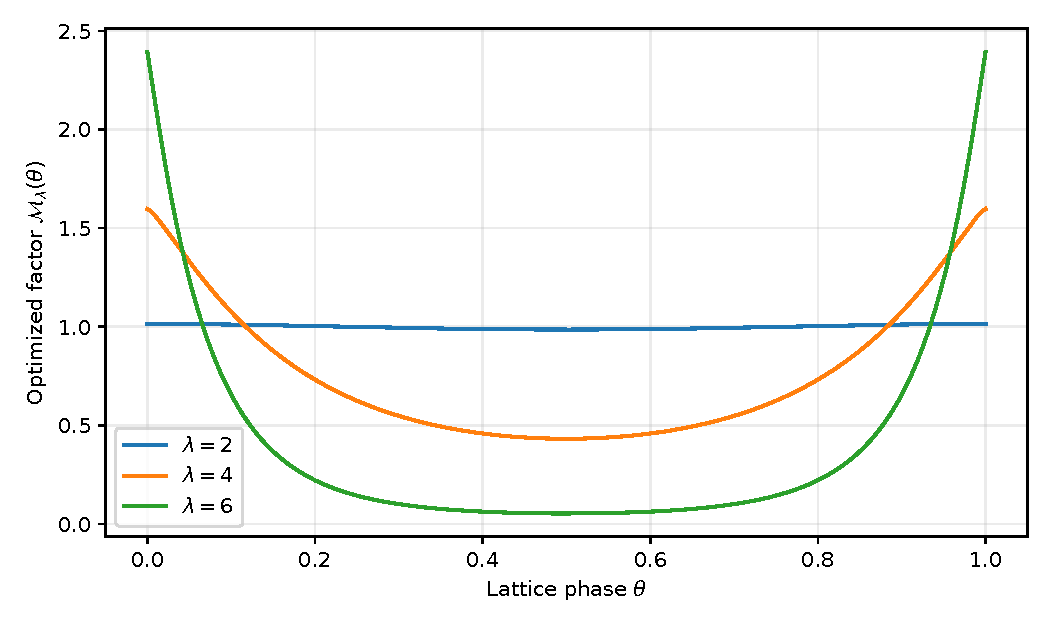
\includegraphics[width=.87\textwidth]{figures/optimized_theta.pdf}
\caption{The optimized theta factor. The mesh and phase survive in the
leading remainder; replacing the sum by its integral would give the
constant function $1$. This plot illustrates the exact profile definition,
not a numerical proof of the asymptotic theorem.}
\label{fig:theta}
\end{figure}

\subsection{Fixed-mesh experiments}
For $h=2\pi/2.25$ and $h=4$, we compare
$\e^{I_hz}\min_K\calE_0(2K;h,x)$ with the exact two-point-grid minimum
in \eqref{eq:fixed-min}. The rapidly decreasing relative difference is
consistent with an exponentially small omitted contribution.
\begin{center}
\small\begin{tabular}{rrrrr}
\toprule
$h$ & $z$ & $I_h$ & $K_{\min}$ & two-atom rel. error\\
\midrule
2.79253 & 10 & 6.3962511 & 34 & 4.85e-05 \\
2.79253 & 25 & 6.3962511 & 86 & 3.7e-10 \\
2.79253 & 60 & 6.3962511 & 206 & 9.58e-23 \\
4.00000 & 10 & 6.6059845 & 30 & 6.38e-08 \\
4.00000 & 25 & 6.6059845 & 73 & 6.88e-19 \\
4.00000 & 60 & 6.6059845 & 174 & 4.07e-44 \\
\bottomrule
\end{tabular}

\end{center}
The slight oscillation in the scaled minimum itself is retained in the
CSV. It is described by the shifted step-two grid, and is not an error
that should be averaged away.

\begin{figure}[htbp]
\centering
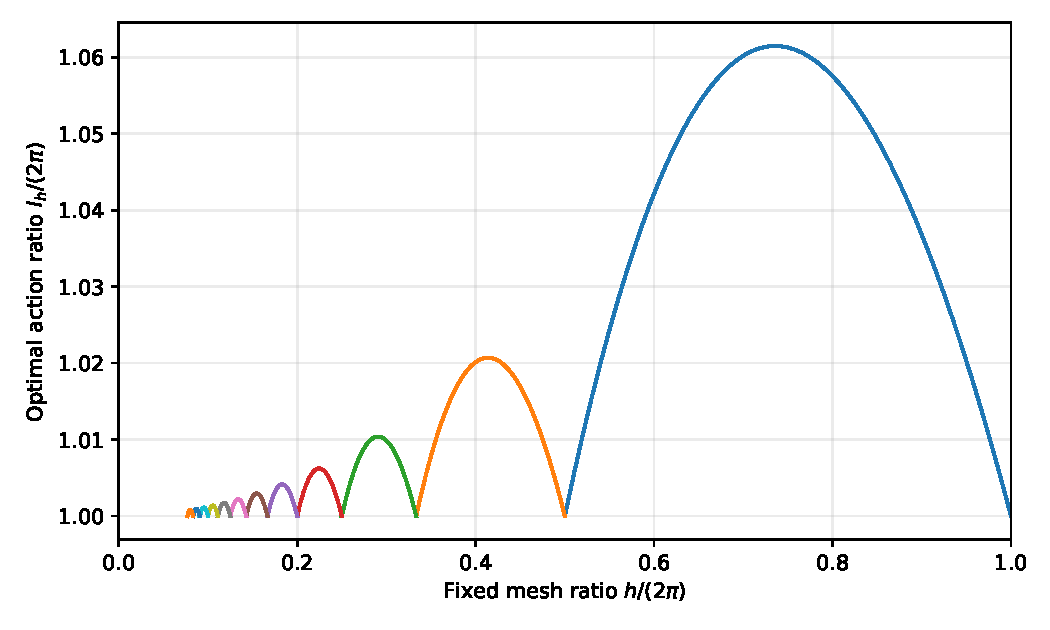
\includegraphics[width=.87\textwidth]{figures/arithmetic_action.pdf}
\caption{The fixed-mesh action $I_h/(2\pi)$ for the ordinary remainder.
It is strictly greater than $1$ between resonances and equals $1$ at
$h/(2\pi)=1/n$. The theorem applies on the open nonresonant intervals;
Proposition~\ref{prop:resonance} treats their resonant endpoints.}
\label{fig:action}
\end{figure}

\subsection{Pole resolution and checks not claimed}
Three additional cases resolve $L=0,1,2$ poles while keeping the same
scaled mesh and phase. They give the same normalized leading theta law,
with the expected replacement of $\beta$ by $2\pi(L+1)$. The receipt
records all 15 critical-mesh cases, six fixed-mesh cases, and three
pole-resolution cases, with all assertions passing.

The experiments do not establish the all-order theorem, do not verify
complex Stokes data, and do not prove a claim about an arbitrary analytic
interpolation. Their purposes are to detect signs, normalization mistakes,
order-rounding errors, and a failed asymptotic prediction. The mathematical
justification is given in the preceding proofs.

\section{Interpretation for the transseries program}
\label{sec:interpretation}

\subsection{Three distinct levels of asymptotic information}
For this family, the following levels should not be conflated.

\paragraph{Formal coefficients.}
The Bernoulli--polylogarithm expressions determine every fixed-order
coefficient. They do not by themselves determine the size of a remainder
when the number of terms grows with $x$.

\paragraph{A specified near-least-term remainder.}
The rule $2K=\beta z+O(1)$ produces a theta factor
$\Theta_\lambda(\theta)$. This gives the lattice-to-integral transition,
but it is still the error of a specified rule.

\paragraph{The actual minimum and a refined representation.}
Minimization changes the leading factor to $\calM_\lambda(\theta)$ and
usually shifts the order by $\sqrt z$. At fixed nonresonant mesh, the
action changes to $I_h$. Resolving exact pole components changes the
representation itself and moves the first unresolved action to a larger
$\beta$. These are different operations and have different certificates.

The results illustrate why a single statement that an expansion is
``Gevrey'' or ``optimally truncated'' can conceal important information.
The index convention, lattice scale, phase, representation, and domain of
uniformity all need to be specified. In particular, the improved action
$I_h$ does not contradict the location of the first formal Borel pole:
the parameter-dependent coefficients and their discrete sampling remain
part of the truncation problem.

\subsection{What remains outside the theorem package}
No theorem here supplies a universal resurgent completion of a Hahn field,
a general composition theorem for exponential transseries, or a global
complex Stokes classification. We do not prove that these theta
coefficients belong to the repository's original two-generator
polynomial--logarithmic algebra. They naturally record a moving lattice
phase and are an analytic extension of the error analysis.

The fixed-mesh result assumes $0<h<\beta$ and excludes exact resonances.
The critical-mesh result keeps $\lambda$ bounded. The overlap result
requires all three scale conditions in \eqref{eq:overlap-assumptions} and
phase separation from resonance. The pole count and the ray are fixed.
These restrictions are explicit mathematical hypotheses, not cosmetic
qualifications.

\subsection{A realistic formalization route}
A useful first formalization target is smaller than the complete article.
The finite geometric identity, positivity of $W$, and the partial-order
comparison of truncated positive sums give a direct certificate layer.
The variance identity and increasing neighboring ratios supply a global
optimization certificate without formalizing theta functions.

The next layer is real analysis: the integral and lattice tail bounds,
the slope theorem, and residual-to-inverse transport. These fit the
repository's stated separation between coefficient identities and analytic
remainder transport \cite{repo-canonical}. Only afterward is it necessary
to formalize Gaussian lattice domination, the differentiable uniform
saddle expansion, and the zero-mean tilt. The pole hierarchy is then a
parameterized reuse of the same theorem rather than a separate proof for
every $L$.

No Lean source is included because none was compiled for this work.
A symbolic equality in the verification script is not described as a
kernel-checked theorem.

\section{Further research questions and topics}
\label{sec:questions}

The following are precisely delimited next questions. They are not being
advertised as established open problems throughout the published
literature; a dedicated priority review would be needed for that claim.

\begin{enumerate}[leftmargin=*,label=\textbf{Q\arabic*.},itemsep=7pt]
\item \textbf{The optimized resonance boundary layer.}
Determine a uniform minimum when $\lambda\to\infty$ and
$\theta\to0$ simultaneously. The entropy formula of
Proposition~\ref{prop:largetheta} is not uniform there. At exact resonance
an order-independent lattice contribution dominates, and subordinate
poles and neighboring lattice points choose the optimal order. Find the
scales at which those mechanisms exchange control.

\item \textbf{The complete fixed-$h$ phase diagram for $h\ge\beta$.}
There is no lattice point below the first unresolved pole in this regime.
Determine the limiting optimal integer order and all transition values of
$h$. The exact positive moment representation reduces the question to a
well-defined family of kernel comparisons, but the two-point chord
argument of Theorem~\ref{thm:fixed} no longer applies unchanged.

\item \textbf{Coalescing ray parameters.}
Allow $(a_j-a_*)x$ to stay bounded while $x\to\infty$. The multiplicity
$m_*$ should be replaced by a finite weighted collection of nearly
minimal rays. Determine the accompanying changes to the tilt, bounded
order correction, and exponential separation estimates, with explicit
uniformity in the ray parameters.

\item \textbf{A growing number of resolved poles.}
Let $L=L(x)\to\infty$. Identify the largest growth range in which a
uniform version of the pole hierarchy remains useful. The denominator
scale, saddle width, pole-separation estimate, and cost of evaluating the
resolved correction must be controlled together; the present fixed-$L$
statement does not settle this problem.

\item \textbf{Optimal computational cost rather than optimal truncation.}
Choose $K$, $L$, the lattice cutoff, pole cutoff, and working precision to
minimize total cost at a required certified accuracy. This requires a
condition-number analysis of the combined kernels, not only a small
mathematical remainder. A positive-kernel formulation may avoid much of
the cancellation in $T_K$ plus the resolved correction.

\item \textbf{A fully validated implementation.}
Implement outward-rounded versions of Theorem~\ref{thm:finite} and
Lemma~\ref{lem:convex}, including theta-root enclosures and a robust
near-tie test for adjacent truncation orders. The existing code provides
reproducible diagnostics, but arithmetic certification remains a distinct
engineering and proof task.

\item \textbf{Complex sectors and Stokes data.}
Continue the positive real-axis formulas to specified complex sectors
and determine which theta factors survive contour deformation. Positivity
and real convexity are essential in the present optimization proof; their
complex replacements need to be stated rather than assumed. Any relation
to the known quantum-dilogarithm Stokes structure should be made at the
level of an explicit normalization.

\item \textbf{Signed or oscillatory analogues.}
For factorial quotients whose analogue of $W$ changes sign, determine
conditions that preserve a useful optimization principle. Leading-ray
cancellation can move the action and destroy log-convexity. A criterion
in terms of the signed spectral measure would extend the method beyond
positive multinomial rays.

\item \textbf{A sharp inverse transseries, not only an enclosure.}
Combine the theta-resolved residual with an all-order expansion of
$F_h'$ and its higher derivatives to obtain phase-dependent inverse-error
coefficients. The present slope bound gives a reliable enclosure, but it
does not yet identify the sharp leading constant for every inverted
parameter regime.

\item \textbf{A reusable formal saddle-to-lattice theorem.}
Formalize a theorem for positive sums with a moving nondegenerate saddle,
a bounded scaled mesh, and a differentiable order parameter. Show how the
zero-mean tilt and neighboring-ratio certificate can be exported as a
common interface for other transseries in ProveIt, without constructing
an unnecessarily broad formal transseries field first.
\end{enumerate}

\section{Conclusion}
The lattice-to-integral question has two answers, depending on what is
being optimized. A prescribed near-least-term rule gives an ordinary
theta factor. The exact minimum over all truncation orders gives a tilted
theta factor, with an explicit $\sqrt x$ displacement and a calculable
bounded correction. At fixed nonresonant mesh, a logarithmic-mean chord
produces a strictly larger action and a residual integer-order oscillation.
A direct overlap theorem connects the two descriptions.

The same proof works after resolving any fixed number of partial-fraction
poles. This yields a concrete, signed, and finitely certifiable hierarchy
of more accurate approximations and inverse enclosures. The resulting
extension is narrower than a general theorem about resurgence, but it is
substantive: it determines errors and optimal orders that fixed-order
formal coefficients alone do not reveal.

\appendix
\section{An explicit coefficient-generation recurrence}
\label{app:recurrence}

For implementability, the generating rule \eqref{eq:Pgen} can be written
using only polynomial arithmetic. Let
\begin{align}
 A(\eps,u)&=\frac1{1+\eps u+\eps^2u^2/2}
             =\sum_{n\ge0}a_n(u)\eps^n,\\
 a_0&=1,\qquad a_1=-u,\qquad
 a_n=-u a_{n-1}-\tfrac12u^2a_{n-2}\quad(n\ge2),\\
 E_j(u,\eta)&=\frac{(-1)^{j+3}u^{j+2}}{j+2}
            +\frac{\eta(-1)^{j+2}u^{j+1}}{j+1}\quad(j\ge1),\\
 H(\eps,u,\eta)&=\exp\left(\sum_{j\ge1}E_j\eps^j\right)
                    =\sum_{n\ge0}h_n(u,\eta)\eps^n.
\end{align}
Differentiating $H$ formally gives the recurrence
\begin{equation}
 h_0=1,\qquad nh_n=\sum_{j=1}^n jE_jh_{n-j},\qquad
 P_n=\sum_{j=0}^n a_jh_{n-j}.
 \label{eq:polyrec}
\end{equation}
This proves finiteness of every coefficient and gives an elementary
algorithm for arbitrarily many saddle corrections. Averaging each
monomial $u^j$ is equivalent to applying $\partial_\eta^j$ to $\calJ$.
Thus the all-order expansion can be represented using a finite collection
of theta derivatives at every requested order.

For a bounded unscaled offset $\sigma$ instead of a bounded tilt, multiply
$Q_\eps(u,0)$ by $(1+\eps u)^\sigma$. This produces the endpoint-offset
polynomials used in Corollary~\ref{cor:endpoint}. These are coefficient
identities; the analytic remainder in the resulting expansion still comes
from Theorem~\ref{thm:theta}, not from the recurrence alone.

\section{Claim ledger and provenance}
\label{app:ledger}

\begin{longtable}{@{}>{\raggedright\arraybackslash}p{.23\textwidth}>{\raggedright\arraybackslash}p{.43\textwidth}>{\raggedright\arraybackslash}p{.27\textwidth}@{}}
\toprule
Result & Content & Status in this article\\\midrule
\endfirsthead
\toprule Result & Content & Status in this article\\\midrule\endhead
Exact positive remainder & Bernoulli kernel, signed multinomial weight,
continuous endpoint & Starting mechanism rederived; not claimed new\\[4pt]
Theorem~\ref{thm:theta} & All-order critical-mesh expansion with phase and
order tilt, including derivatives & Developed and proved here\\[4pt]
Theorem~\ref{thm:optimal} & Global minimization, $\sqrt z$ order shift,
bounded order correction, first minimum correction & Developed and proved here\\[4pt]
Corollary~\ref{cor:endpoint} & Explicit $-13/24$ coefficient and integer
order oscillation & Derived refinement\\[4pt]
Theorem~\ref{thm:fixed} & Logarithmic-mean action, strict action improvement,
periodic order prefactor & Developed and proved here\\[4pt]
Theorem~\ref{thm:overlap} & Direct mesoscopic matching theorem & Developed
and proved here\\[4pt]
Theorem~\ref{thm:hierarchy} & Reoptimized, exactly pole-resolved hierarchy &
Developed and proved here from the same kernel\\[4pt]
Finite and inverse certificates & Positive-sum truncation and slope-based
transport & Explicit reusable estimates; conditioning rederived\\[4pt]
General resurgence, complex Stokes data, growing $L$ & Wider analytic
extensions & Not established here\\
\bottomrule
\end{longtable}

The inspected earlier manuscript is identified by filename
\path{uniform_q_multinomial_transseries.tex}, dated 29 September 2026,
1,521 source lines in its saved version. Its equation labels
\texttt{eq:Rexact}, \texttt{eq:Rzero}, \texttt{eq:discrete-remainder}, and
\texttt{thm:resonance}, together with Question~1 and Question~2 of its
further-research section, specify the comparison. Its content was read,
not inferred from its abstract alone. The separate saved manuscript on a
uniform resurgent crossover and the saved one-exponential reversion
manuscript were checked at the scope/abstract level to avoid presenting
their principal results as new results of this article.

The repository READMEs distinguish exact formalization from partial
interfaces and absent assembled analytic developments. This article
preserves that distinction. It does not infer machine verification from
a README inventory, and it does not assert commit-to-PDF publication
parity for a repository render that was not inspected.

\section{Reproduction and file inventory}
\label{app:reproduction}

The package contains the editable source \texttt{article.tex}, the compiled
\texttt{article.pdf}, two figure files with their plotting script, the
verification script, CSV data, generated numerical tables, a JSON receipt,
and a source/claim audit. From the package directory:
\begin{verbatim}
python -m pip install -r requirements.txt
python code/verify.py
python code/plots.py
pdflatex -interaction=nonstopmode -halt-on-error article.tex
pdflatex -interaction=nonstopmode -halt-on-error article.tex
pdflatex -interaction=nonstopmode -halt-on-error article.tex
\end{verbatim}
The shipped figures and tables allow rebuilding the PDF without rerunning
the numerical scripts. The tests contain no network calls and do not
modify the ProveIt repository. The manuscript has been compiled and its
rendered pages inspected; that document-production check is separate from
mathematical verification.

\begin{thebibliography}{99}
\bibitem{repo}
V. Reshetnikov, \emph{ProveIt}, research and formalization repository.
\url{https://github.com/VladimirReshetnikov/ProveIt}.
Accessed 29 September 2026.

\bibitem{repo-group}
ProveIt, \emph{Series and transseries group README}, pinned source at commit
\texttt{ae28ea2db3c01a0b777cffa6295b8fe9c4628f27}.
\url{https://github.com/VladimirReshetnikov/ProveIt/blob/ae28ea2db3c01a0b777cffa6295b8fe9c4628f27/Analysis/FabiusFunction/docs/semi-formalized-research-frontiers/drafts/series-and-transseries/README.md}.
% ed. (2026-09-29): current path added by ProveIt.
Editorial note (ProveIt, 2026-09-29): pre-split path; the group README is now
\path{Analysis/Transseries/docs/series-and-transseries/README.md}.

\bibitem{repo-canonical}
ProveIt, \emph{Transseries and Inversion: package README}, same pinned
commit, statement-level formalization inventory and source boundary.
\url{https://github.com/VladimirReshetnikov/ProveIt/blob/ae28ea2db3c01a0b777cffa6295b8fe9c4628f27/Analysis/FabiusFunction/docs/semi-formalized-research-frontiers/drafts/series-and-transseries/Transseries_And_Inversion/README.md}.
% ed. (2026-09-29): current path added by ProveIt.
Editorial note (ProveIt, 2026-09-29): pre-split path; that README is now
\path{Analysis/Transseries/docs/series-and-transseries/Transseries_And_Inversion/README.md}.

\bibitem{prior}
OpenAI, \emph{Uniform $q$-Multinomial Transseries and Certified Inversion:
Closing the $q\to1$ endpoint gap, locating Borel singularities, and proving
a sharp least-term exponential rate}, research draft prepared for
Vladimir Reshetnikov, 29 September 2026. User-provided saved research
source, \path{uniform_q_multinomial_transseries.tex}; especially the
positive remainder and Further Research Questions~1--2. Unrefereed.
% ed. (2026-09-29): filed path added by ProveIt.
Editorial note (ProveIt, 2026-09-29): now filed as
\path{Analysis/Transseries/docs/series-and-transseries/Uniform_q_Multinomial_Certified_Inversion/uniform_q_multinomial_transseries.tex}.

\bibitem{dlmf-hyperbolic}
NIST Digital Library of Mathematical Functions, \S4.36,
\emph{Infinite Products and Partial Fractions}, particularly (4.36.3).
\url{https://dlmf.nist.gov/4.36}.

\bibitem{dlmf-gamma}
NIST Digital Library of Mathematical Functions, \S5.9,
\emph{Integral Representations}, Binet and polygamma integrals.
\url{https://dlmf.nist.gov/5.9}.

\bibitem{dlmf-qgamma}
NIST Digital Library of Mathematical Functions, \S5.18,
\emph{$q$-Gamma and $q$-Beta Functions}, definitions and limiting values.
\url{https://dlmf.nist.gov/5.18}.

\bibitem{dlmf-theta}
NIST Digital Library of Mathematical Functions, \S20.7(viii),
\emph{Transformations of Lattice Parameter}, particularly (20.7.32).
\url{https://dlmf.nist.gov/20.7.viii}.

\bibitem{discrete-laplace}
J. A. Hughes, J. W. Helton, and P. Schlosser,
\emph{The discrete Laplace asymptotic method and its application to the
3XOR satisfiability problem}, arXiv:2509.16420, 2025.
Version 1 consulted for the general discrete Laplace framework.
\url{https://arxiv.org/abs/2509.16420}.

\bibitem{costin-garoufalidis}
O. Costin and S. Garoufalidis,
\emph{Resurgence of the Euler--MacLaurin summation formula},
arXiv:math/0703641, 2007.
\url{https://arxiv.org/abs/math/0703641}.

\bibitem{garoufalidis-kashaev}
S. Garoufalidis and R. Kashaev,
\emph{Resurgence of Faddeev's quantum dilogarithm},
arXiv:2008.12465, 2020.
\url{https://arxiv.org/abs/2008.12465}.
% ed. (2026-09-29): editorial bibliography entries added by ProveIt.
\bibitem{ed:siblings}
[Editorial addition, ProveIt, 2026-09-29.] The five packages of the
$q\to1$ merge unit in the ProveIt series-and-transseries collection,
\path{Analysis/Transseries/docs/series-and-transseries/}:
\path{Uniform_q_Multinomial_Certified_Inversion/uniform_q_multinomial_transseries.tex};
\path{Uniform_Resurgent_Crossover_Gaussian_Binomials/article.tex};
\path{Certified_Inversion_q_to_1_Transition/q_transition.tex};
\path{Gamma_Core_q_to_1_Crossover/Gamma_Core_Transseries.tex};
\path{Theta_Resolved_Optimal_Truncation_q_Multinomial/article.tex}.
Filed in batches 45 and 46 of \path{docs/incoming/README.md}; unrefereed.

\bibitem{ed:gcc}
[Editorial addition, ProveIt, 2026-09-29.] ProveIt, \emph{Gaussian
Coefficient Calculus},
\path{Analysis/FabiusFunction/docs/semi-formalized-research-frontiers/drafts/combinatorial-coefficient-calculus/Gaussian_Coefficient_Calculus/Gaussian_Coefficient_Calculus.tex},
Theorem \texttt{q3:thm:double-scaling} (line 3942) and its domain
\texttt{q3:eq:double-scaling-domain}.

\bibitem{ed:tai}
[Editorial addition, ProveIt, 2026-09-29.] ProveIt, \emph{Transseries: the
polynomial-logarithmic calculus, series reversal at infinity, and
inversion} (canonical volume),
\path{Analysis/Transseries/docs/series-and-transseries/Transseries_And_Inversion/transseries_and_inversion.tex},
Theorem \texttt{p0:thm:optimal-truncation} (line 39360).

\bibitem{ed:lean}
[Editorial addition, ProveIt, 2026-09-29.] ProveIt Lean library:
\path{Fabius.exists_eq_in_residual_interval} in
\path{Analysis/FabiusFunction/Lean/FabiusFunction/MeanValueBracket.lean}
and \path{Fabius.transport_bound} (the crosswalk of the canonical volume's
\texttt{p0:eq:transport-bound}) in
\path{Analysis/FabiusFunction/Lean/FabiusFunction/RemainderTransport.lean}.
\end{thebibliography}
\end{document}
